\documentclass[11pt]{article}
\usepackage[a4paper,margin=2.2cm]{geometry}
\usepackage{graphicx,booktabs,amsmath,amssymb,xcolor,caption,tabularx,array,enumitem,adjustbox,multirow}
\usepackage[hidelinks]{hyperref}
\usepackage{mathptmx}
\captionsetup{font=small,labelfont=bf}
\setlength{\parskip}{3pt}
\newcolumntype{Y}{>{\raggedright\arraybackslash}X}
\newenvironment{revcomment}{\begin{quote}\itshape}{\end{quote}}
\newcommand{\answerhead}[1]{\par\medskip\noindent\textbf{#1}\par}
\title{\vspace{-1.4cm}McQueenGuard: Learning-Assisted Verification Framework for Runtime Safety Assurance of Self-Driving Systems (JSA-D-26-01243)\\[4pt]
\large Responses and additional experiments for Reviewer~\#1 (Comments~6 and 7) and Reviewer~\#2 (Comments~6 and 7)}
\date{}
\begin{document}
\maketitle
\vspace{-1.3cm}
\noindent This document contains (Part~I) the answers to the four comments for the revision letter and (Part~II) the new
material for Section~6 of the manuscript. The comparison, ablation and out-of-distribution analyses (Sections~6.9--6.11) share one set of experiments: all methods
and ablation variants were run on the same <<N_EP>> scenario instances. The embedded-timing and sensor-noise shift experiments of
Section~6.12 are separate runs with the same scenario generator.
Table and figure numbers continue the numbering of the manuscript (the last table in Section~6 is Table~5 and the last figure is
Figure~17); the comparison table of Section~7 (currently Table~6) becomes Table~19.

\tableofcontents

%=====================================================================================================
\part*{Part I \quad Answers for the revision letter}
\addcontentsline{toc}{part}{Part I \quad Answers for the revision letter}

\section*{Reviewer \#1, Comment 6}
\addcontentsline{toc}{section}{Reviewer \#1, Comment 6}
\begin{revcomment}
``Could you supplement the desktop-based experiments with latency, memory footprint, and power consumption data when deploying
the MLP verifier on an automotive-grade embedded platform (e.g., NVIDIA Orin)? How would the framework handle domain adaptation
challenges, such as simulation-to-real shifts in sensor noise distributions, to substantiate claims of embedded system
applicability?''
\end{revcomment}
\answerhead{Answer:}
We thank the reviewer for this suggestion. We have added a deployment study and a sensor-noise shift study to the revised
manuscript (please see the new Section~6.12, Tables~\ref{tab:emb}--\ref{tab:sc} and Figures~\ref{fig:et}--\ref{fig:ss}).

\emph{Embedded profile.} The learned verifier has <<f"{mod['params']:,}">> parameters (<<f"{mod['fp32_kib']:.0f}">>\,KiB in
FP32, <<f"{mod['onnx_int8_kib']:.0f}">>\,KiB as an INT8 ONNX model) and needs <<f"{mod['macs']:,}">> multiply-accumulate
operations per inference. On one CPU thread, MLP inference takes <<us(LB['mlp_onnx_fp32']['mean_us'])>> with ONNX Runtime and
a complete learned decision (feature extraction, inference, familiarity check, admission test and action selection) takes
<<us(pth['mean_us'])>> on average (<<us(pth['p99_us'])>> at the 99th percentile), compared with <<f"{qx['mean']:.0f}">>\,ms for exact
verification with PRISM. A minimal inference process occupies <<f"{mem['ort_int8_process']:.0f}">>\,MB of resident memory,
of which the inference session accounts for <<f"{mem['ort_int8_session_increment']:.0f}">>\,MB; the PRISM verification
server occupies up to <<f"{mem['prism_jvm_peak_rss']:.0f}">>\,MB. We did not have access to an NVIDIA Orin board during the
revision. We therefore report projected latencies for the Arm Cortex-A78AE CPU of the Jetson AGX Orin under an explicit
1.5--4$\times$ single-thread slow-down band, and an upper bound on the energy per decision derived from the 15--60\,W module
power envelope (<<f"{proj['central']['energy_upper_mJ']['15 W']['learned']:.1f}">>--<<f"{proj['central']['energy_upper_mJ']['MAXN 60 W']['learned']:.1f}">>\,mJ for a
learned decision versus <<f"{proj['central']['energy_upper_mJ']['15 W']['exact']/1000:.0f}">>--<<f"{proj['central']['energy_upper_mJ']['MAXN 60 W']['exact']/1000:.0f}">>\,J for an exact
verification at the central slow-down). These are projections, not measurements, and we state this in the manuscript. To check
whether the closed-loop results survive slower hardware, we re-ran <<n_et>> paired episodes with every computation time
multiplied by 2.5. The learned decision path remained far below the 100\,ms decision period, but McQueenGuard's safety
violations rose from <<f"{ETd[(MQ,'desktop')].margin_violation:.0f}">>\,\% to <<f"{ETd[(MQ,'embedded')].margin_violation:.0f}">>\,\%
(<<int(round(ETd[(MQ,'embedded')].margin_violation-ETd[(MQ,'desktop')].margin_violation))>> more of <<n_et>> episodes, an indicative rather than significant
difference), consistent with each fallback waiting longer for PRISM. On an embedded platform the exact verifier is therefore the bottleneck, and we
discuss running it on a dedicated core with a bounded model size.

\emph{Sensor-noise shift.} We evaluated an unannounced shift of the perception noise model (heavy-tailed noise, a systematic
bias, additional drop-outs and latency, at three severity levels). Three mechanisms of the framework act under such a shift:
the familiarity check routes unfamiliar inputs to exact verification; the exact results of these fallbacks are fed back to
recalibrate the error margin over a rolling window (Algorithm~1, lines~27--28), complemented by shadow audits of 10\,\% of the
admitted decisions; and the Simplex shield remains active independently of the learned verifier. Under the shift the
coverage of the offline margin varied between <<f"{100*min(SS[k]['coverage_static'] for k in SS):.1f}">> and <<f"{100*max(SS[k]['coverage_static'] for k in SS):.1f}">>\,\%
(<<f"{100*ss1['coverage_static']:.1f}">>\,\% at the highest severity), and the unsafe-admission rate of the static margin rose from <<f"{100*ss0['static_gate']['unsafe_admission_rate']:.1f}">>\,\% to
<<f"{100*ss1['static_gate']['unsafe_admission_rate']:.1f}">>\,\% of admitted decisions. With recalibration the margin grew from
<<f"{R2['eps']:.3f}">> to <<f"{ss1['adaptive_gate']['eps_final']:.3f}">> and the unsafe-admission rate remained between
<<f"{100*min(SS[k]['adaptive_gate']['unsafe_admission_rate'] for k in SS):.1f}">> and <<f"{100*max(SS[k]['adaptive_gate']['unsafe_admission_rate'] for k in SS):.1f}">>\,\% across the severities, at the cost of admitting fewer decisions
(<<f"{100*ss1['adaptive_gate']['admission_rate']:.0f}">>\,\% instead of <<f"{100*ss1['static_gate']['admission_rate']:.0f}">>\,\%).
Recalibration does not restore exchangeability, so under a persistent shift the statistical statement remains conditional on the
recalibration window; we state this in Section~6.13 and list on-vehicle validation as future work. The ONNX models and the
benchmarking scripts are included in the project repository so that the measurements can be repeated on the target hardware.

\section*{Reviewer \#1, Comment 7}
\addcontentsline{toc}{section}{Reviewer \#1, Comment 7}
\begin{revcomment}
``Could you expand the baseline comparisons to include (1) other learning-assisted verification frameworks (e.g., VerifAI),
(2) conventional autonomous driving planners (e.g., MPC, rule-based methods), and (3) end-to-end reinforcement learning planners
to better highlight McQueenGuard's advantages in safety assurance and real-time efficiency?''
\end{revcomment}
\answerhead{Answer:}
We thank the reviewer for this suggestion. We have added a closed-loop comparison (please see the new Sections~6.8 and 6.9,
Tables~\ref{tab:methods}--\ref{tab:c7b} and Figures~\ref{fig:c7a}--\ref{fig:c7c}) with (1) a VerifAI-based runtime-assurance
pipeline (falsification with VerifAI's cross-entropy sampler, a learned violation monitor and Simplex switching to a braking
controller), (2) the collision-avoidance MPC of Zhang et al.\ (IEEE T-ITS, 2022) and a rule-based planner (Intelligent Driver
Model with emergency braking), and (3) an end-to-end PPO planner trained with a CaRL-style reward. McQueenGuard with exact
verification at every decision is included as a reference. All methods ran on the same <<N_EP>> scenario instances (<<N_PER_CAT>>
per scenario category of Table~3). McQueenGuard had a collision rate of <<f1(O[MQ]['collision'])>>\,\% and a safety-violation rate
(collision or violation of the 2\,m safe margin) of <<f1(O[MQ]['margin_violation'])>>\,\%, compared with
<<f1(O[VA]['margin_violation'])>>\,\% for VerifAI, <<f1(O[MP]['margin_violation'])>>\,\% for MPC, <<f1(O[RB]['margin_violation'])>>\,\%
for the rule-based planner and <<f1(O[PP]['margin_violation'])>>\,\% for end-to-end PPO. <<C7_SIG_SENTENCE>> <<C7_COL_SENTENCE>> <<C7_RISK_SENTENCE>> McQueenGuard is the only method that attaches a
calibrated error bound to each admitted decision. With respect to
real-time efficiency, <<f"{O[MQ]['learned_share']:.0f}">>\,\% of McQueenGuard's decisions were taken by the learned verifier in
microseconds, which reduced the mean decision latency from <<f"{O[EX]['lat_mean']:.0f}">>\,ms (exact verification at every
decision) to <<f"{O[MQ]['lat_mean']:.0f}">>\,ms and the share of decisions missing the 100\,ms decision period from
<<f"{O[EX]['miss']:.0f}">>\,\% to <<f"{O[MQ]['miss']:.0f}">>\,\%. The comparison also shows the costs of the approach, which we
report in the manuscript: McQueenGuard is more cautious than MPC and the rule-based planner (median travel-time ratio
<<f2(O[MQ]['delay_ratio'])>> against <<f2(O[MP]['delay_ratio'])>> and <<f2(O[RB]['delay_ratio'])>>), the remaining
violations occur mainly while a fallback waits for PRISM and in the novel-trajectory category, whose occluded and running
pedestrians are not represented in the verification model, and VerifAI reached a <<VA_VS>> violation rate but deadlocked in
<<f1(O[VA]['deadlock'])>>\,\% of the episodes.

\section*{Reviewer \#2, Comment 6}
\addcontentsline{toc}{section}{Reviewer \#2, Comment 6}
\begin{revcomment}
``The experimental evaluation demonstrates substantial latency reduction and relatively small approximation errors, but it could
be strengthened in two aspects. First, an ablation study is needed to distinguish the contribution of the learned verifier from
that of the proposed error-aware admission and exact fallback mechanisms. The evaluation should also provide larger-scale
evidence on decision preservation and safety outcomes rather than relying mainly on illustrative cases.''
\end{revcomment}
\answerhead{Answer:}
We thank the reviewer for this valuable comment. We have added an ablation study and a large-scale preservation analysis
(please see the new Section~6.10, Tables~\ref{tab:abl}--\ref{tab:th1} and Figures~\ref{fig:abl}--\ref{fig:pres}).

\emph{Ablation.} Starting from the complete framework, we removed one component at a time: the conformal margin, the
familiarity check, the exact fallback (replaced by the conservative fallback control), the whole admission mechanism (learned
verifier only), the Simplex shield, and the learned verifier itself (exact verification only). Each variant ran on the same
<<N_EP>> scenario instances (<<f"{len(ABL_PRESENT)*N_EP:,}">> closed-loop runs in total, including the idealised reference described below). The results separate the
contributions as follows. The learned verifier is what makes runtime verification feasible: with exact verification at every
decision, <<f"{A[EX]['miss']:.0f}">>\,\% of the decisions missed the 100\,ms decision period and the safety-violation rate was
<<f1(A[EX]['margin_violation'])>>\,\% (<<f1(A[MQ]['margin_violation'])>>\,\% for the complete framework). The error-aware admission
controls how often a learned result is wrongly admitted: on the exactly verified decision stream, the share of decisions in
which an action with exact unsafe probability $\ge\theta$ was admitted fell from <<f2(POL['ID']['learned']['false_adm_per_dec'])>>\,\% to
<<f2(POL['ID']['full']['false_adm_per_dec'])>>\,\% in-distribution and from <<f2(POL['OOD']['learned']['false_adm_per_dec'])>>\,\% to
<<f2(POL['OOD']['full']['false_adm_per_dec'])>>\,\% out of distribution, and in closed loop the margin reduced the share of executed
commands with verified risk above $\theta$ from <<f1(A[NOEPS]['risk_violation'])>>\,\% to <<f1(A[MQ]['risk_violation'])>>\,\%.
The exact fallback is what keeps the vehicle making progress when the learned verifier is not admitted: replacing it by the
conservative fallback control gave the lowest violation rate (<<f1(A[NOEXACT]['margin_violation'])>>\,\%) but
<<f1(A[NOEXACT]['deadlock'])>>\,\% deadlocks, including every episode of the high-noise and unseen-weather categories. Removing the
Simplex shield raised the safety-violation rate to <<f1(A[NOMON]['margin_violation'])>>\,\% (<<pfmt(R2['ablation_mcnemar_mv'][NOMON][2])>>),
because the shield covers the interval in which an exact result is pending. The deployable variants with fewer violations than the complete
framework either deadlocked more often or had no bound on false admissions, so no single component can be removed without losing
liveness, safety or the statistical guarantee. <<IDEAL_SENTENCE>>

\emph{Larger-scale preservation evidence.} Instead of the twelve illustrative cases of Table~2, every third decision of the
complete framework in all <<N_EP>> episodes was additionally verified exactly for all candidate actions
(<<f"{n_dec_total:,}">> decisions). Safety preservation holds at this scale within the stated statistical bound: false admissions
occurred in <<f2(POL['all']['full']['false_adm_per_dec'])>>\,\% of all decisions and in at most <<f2(all_fa_max)>>\,\% in any
scenario category, below $\alpha=5\,\%$ (Corollary~1). Decision preservation in the sense of Theorem~1 is more limited: the admitted
learned decision coincided with the exact decision in <<f1(R2['admitted_agree'])>>\,\% of the cases. Where it differed, the
learned action was safe in <<f"{100*R2['disagree_safe']/max(1,R2['disagree_total']):.0f}">>\,\% of the cases and more cautious than the
exact action in <<f"{100*R2['disagree_conservative']/max(1,R2['disagree_total']):.0f}">>\,\%, and the mean utility loss was
<<f"{REGRET_DIS:.3f}">> (utilities range from 0 to about 1.3). The sufficient condition of Theorem~1 was
verified at scale (whenever the realised utility error satisfied $2\max_a|U(a)-\hat U(a)|<\mathcal{T}(k)$, the decisions agreed in
<<f1(TH['oracle_pos']['agree'])>>\,\% of <<f"{TH['oracle_pos']['n']:,}">> cases), but with the calibrated utility margin
($\varepsilon_U=<<f"{R2['eps_u']:.3f}">>$) <<CALIB_COND>>, because the utility gap between the best and second-best admissible actions is small (median <<f"{TH['T_median']:.3f}">>).
We have therefore qualified the claims about decision preservation in Sections~5.1, 6.5 and 6.10: the guarantee that matters for
safety is the admission bound, whereas exact agreement of the selected action is not guaranteed in general.

\section*{Reviewer \#2, Comment 7}
\addcontentsline{toc}{section}{Reviewer \#2, Comment 7}
\begin{revcomment}
``Second, the reported empirical error-bound coverage (97.8\%) does not by itself demonstrate that the estimated bound remains
reliable for unknown or out-of-distribution scenarios. The authors should evaluate the error-bound coverage and false-admission
rate under OOD conditions, together with the resulting fallback and safety outcomes. Finally, the reported latency improvement
should clarify whether it represents end-to-end runtime overhead or only learned-model inference time.''
\end{revcomment}
\answerhead{Answer:}
We agree with the reviewer and thank them for this comment. We have added an out-of-distribution evaluation of the error bound
and a latency breakdown (please see the new Section~6.11, Tables~\ref{tab:ood}--\ref{tab:lat} and Figure~\ref{fig:ood}), and we
have extended the sensor-noise shift study of Section~6.12. The learned verifier was trained and calibrated only on the six
in-distribution categories of Table~3; the high-speed, novel-trajectory, high-noise and unseen-weather (snow) categories are out
of distribution. For each category we report the coverage of the calibrated margin, the false-admission rate, the fallback rate
and the closed-loop safety outcomes, all on the decisions taken by the framework itself. The results show that an in-distribution coverage
figure, such as the 97.8\,\% of Table~4 (obtained for the CARLA verifier; our testbed verifier has 94.5\,\%), does not by itself carry over to
shifted conditions:
\begin{itemize}[leftmargin=1.3em,itemsep=1pt]
\item In-distribution, the coverage of the margin over all decisions was <<f1(min(PCd[c].cov_all for c in ID_C))>>--<<f1(max(PCd[c].cov_all for c in ID_C))>>\,\%,
consistent with the nominal 95\,\%. On the subset of risk-relevant decisions it was lower
(<<f1(min(PCd[c].cov_risky for c in ID_C))>>--<<f1(max(PCd[c].cov_risky for c in ID_C))>>\,\%), which illustrates that the conformal guarantee is
marginal rather than conditional. False admissions remained at or below <<f2(id_fa_max)>>\,\% of the decisions.
\item Out of distribution, coverage depends on the type of shift. Under unseen weather it fell to <<f1(PCd['Unseen weather'].cov_all)>>\,\%
(<<f1(PCd['Unseen weather'].cov_risky)>>\,\% on risk-relevant decisions), i.e., the margin is not reliable there. The familiarity check
rejected all high-noise and unseen-weather decisions (fallback rate 100\,\%), so no learned result was admitted in these categories;
without the check, <<f2(PCd['Unseen weather'].fa_dec_nogate)>>\,\% of the unseen-weather decisions would have been false admissions, and
<<f2(PCd['Unseen weather'].fa_dec_learned)>>\,\% without any admission rule. At high speed the fallback rate rose to <<f1(PCd['High speed (50-60)'].fallback)>>\,\% and false admissions stayed at
<<f2(PCd['High speed (50-60)'].fa_dec)>>\,\%. Novel trajectories were not detected as unfamiliar
(<<f1(PCd['Novel trajectory'].familiar)>>\,\% familiar) and the margin remained valid there (<<f1(PCd['Novel trajectory'].cov_all)>>\,\% coverage),
but this category had the highest safety-violation rate of the complete framework (<<f1(PCd['Novel trajectory'].ep_mv)>>\,\%), and exact
verification only reached the same level (<<f1(cmv(EX,'Novel trajectory'))>>\,\%). These violations come from the verification model, which does
not represent occluded or running pedestrians, and not from the learned approximation; the admission rule cannot detect them, and we
now state this limitation explicitly. In the high-speed, high-noise and unseen-weather categories, the remaining violations
(<<f1(PCd['High speed (50-60)'].ep_mv)>>, <<f1(PCd['High noise'].ep_mv)>> and <<f1(PCd['Unseen weather'].ep_mv)>>\,\%, i.e. <<round(PCd['High speed (50-60)'].ep_mv*PCd['High speed (50-60)'].episodes/100)>>, <<round(PCd['High noise'].ep_mv*PCd['High noise'].episodes/100)>> and <<round(PCd['Unseen weather'].ep_mv*PCd['Unseen weather'].episodes/100)>> of <<int(PCd['High noise'].episodes)>> episodes) did not occur when exact
results were made available without delay, which points to the latency of the exact fallback as their cause (significant for the high-speed category,
indicative for the other two).
\item The familiarity check detects shifts of the input distribution (sensor noise, friction outside the training range) but is a
weak predictor of individual bound failures (area under the ROC curve <<f2(R2['gate_auc_all'])>>). It complements, but does not replace,
the online recalibration described in our answer to Reviewer~\#1, Comment~6.
\end{itemize}
\emph{Latency.} The speed-up reported in Table~4 (2.1\,ms against 148.6\,ms) compares the inference time of the learned verifier
with the time of one exact PRISM verification; it is not the end-to-end runtime overhead. We have relabelled these rows and added a
breakdown (Table~\ref{tab:lat}). In our measurements, MLP inference takes <<us(LB['mlp_onnx_fp32']['mean_us'])>>, a complete
learned decision <<us(LB['learned_path']['mean_us'])>> and an exact verification <<f"{LB['prism']['wall_mean_ms']:.0f}">>\,ms, of which
<<f"{check_share:.0f}">>\,\% is model construction and model checking inside PRISM. Because a share of decisions still falls back to
exact verification, the end-to-end reduction of the mean decision latency is <<f"{speedup_e2e:.1f}">>$\times$
(<<f"{O[EX]['lat_mean']:.0f}">>\,ms to <<f"{O[MQ]['lat_mean']:.0f}">>\,ms, <<("an" if str(round(lat_red))[0]=="8" else "a")>> <<f"{lat_red:.0f}">>\,\% reduction), much smaller than the
inference-only ratio; although only <<f"{100-O[MQ]['learned_share']:.0f}">>\,\% of the decisions are exact, they occupy <<f"{TIME_EXACT:.0f}">>\,\% of the driving time,
because each exact verification blocks the planner until it completes. Perception and actuation latencies are the same for all methods and are not included in these figures.

%=====================================================================================================
\clearpage
\part*{Part II \quad New material for Section 6 of the manuscript}
\addcontentsline{toc}{part}{Part II \quad New material for Section 6 of the manuscript}
\setcounter{table}{5}
\setcounter{figure}{17}

\section*{6.8 \quad Extended Closed-Loop Evaluation: Setup}
\addcontentsline{toc}{section}{6.8 Extended closed-loop evaluation: setup}
The experiments in Sections~6.2--6.7 study the framework in CARLA on a limited number of scenarios. To compare McQueenGuard with
alternative approaches and with its own ablations on identical scenario instances, at a scale of thousands of closed-loop runs, and
with computation latency inside the control loop, we use a reproducible closed-loop testbed that re-implements the
pedestrian-crossing scenario of Section~6.1. The testbed is not a substitute for CARLA; its purpose is a controlled, paired
comparison.

\textbf{Scenario.} The ego vehicle (length 4.7\,m) approaches a marked crosswalk from 70\,m at the scenario speed. A pedestrian waits at
the kerb and crosses with probability 0.75, at 1.0--1.8\,m/s, with a hesitation inside the lane in 30\,\% of the crossings; a
pedestrian who waits at the kerb crosses once the vehicle has stopped in front of the crosswalk. The weather presets use the friction,
camera-noise, LiDAR-accuracy and perception-latency values of the CARLA configuration of Section~6. Detection probability decays with
distance and visibility, tracks drop out, positions are measured with noise and arrive after a perception latency of 90--150\,ms, and
actuation has a 0.1\,s delay and a 0.2\,s first-order lag with friction-limited deceleration. Every planner is invoked every 100\,ms,
and its command takes effect only after its own computation time has elapsed; the previous command is held meanwhile.

\textbf{Scenario categories.} We use the ten categories of Table~3, with <<N_PER_CAT>> scenario instances each (<<N_EP>> per method). The six
clear, fog and rain categories are in-distribution: the verified dataset of the learned verifier was collected only in these
categories. The other four are out of distribution: high speed (50--60\,km/h), novel trajectory (running pedestrians, 2.5--3.5\,m/s, or
pedestrians occluded until they step into the road), high noise (three times the measurement noise and 15\,\% additional
drop-outs) and unseen weather (snow, friction about 0.3, visibility about 32\,m).

\textbf{McQueenGuard.} At each decision point the parametric MDP is instantiated with the current valuation $\lambda$ (estimated friction,
perception-error probability, visibility, pedestrian speed, crossing intention and presence belief) and verified for five longitudinal
actions (accelerate, maintain speed, reduce speed, brake, emergency brake) against $P_{\max}{=}?[F^{\le 4\,\mathrm{s}}\,\mathit{unsafe}]$,
where \emph{unsafe} is a collision or a violation of the safe margin $d_{SM}=2$\,m, and the performance reward
$R_{\max}{=}?[C^{\le 4\,\mathrm{s}}]$, with $\theta=0.05$ and the safety-first lexicographic rule of Equations~(16)--(17). Exact
verification uses PRISM~4.8.1 (sparse engine) as a persistent verification server. The learned verifier is the MLP of Section~6.6
(18 inputs; 64, 64 and 32 hidden units), trained on <<f"{V['n_total']:,}">> exactly verified decision points from <<V['n_episodes']>> episodes
(episode-wise 70/15/15\,\% split), with an MAE of <<f"{V['mae_p']:.4f}">> for the unsafe probability and <<f"{V['mae_u']:.4f}">> for the utility. The
split-conformal margin of Equation~(25) at $\alpha=0.05$ is $\varepsilon=<<f"{R2['eps']:.3f}">>$, with <<f1(100*V['coverage_test'])>>\,\% coverage on the
<<f"{V['n_test']:,}">> test decisions (95\,\% interval <<COVCI>>, consistent with the nominal 95\,\%). Because the admitted action is chosen after the estimates are computed, the calibration residual is taken simultaneously over
all candidate actions whose estimate lies below $\theta$, which makes Corollary~1 hold for whichever action is admitted. The familiarity set
$\mathcal{H}$ is implemented as a Mahalanobis-distance test (99th percentile of the calibration set) combined with the training range of every
feature. While an exact result is pending after a non-admitted decision, the fallback safety control (Algorithm~1, line~26) applies at
least the reduce-speed action, and the Simplex shield of Section~4.5 is evaluated every 50\,ms.

\textbf{Metrics.} A \emph{safety violation} is a collision or a gap below $d_{SM}=2$\,m while the pedestrian is in the lane. The \emph{verified
risk} is the share of executed control commands, audited once per second, whose exact 4-s unsafe probability is at least $\theta$; it
includes unavoidable states and is therefore not zero for any method. A \emph{deadlock} is an episode in which the vehicle does not clear the
crosswalk within 30\,s of its free-flow arrival time. The \emph{travel-time ratio} is the time needed to clear the crosswalk divided by the
free-flow time. A \emph{deadline miss} is a decision whose computation exceeds the 100\,ms decision period. Rates are given with 95\,\%
Wilson intervals, and paired differences are tested with exact McNemar tests on the same scenario instances.

\textbf{Hardware.} All timings were measured on one machine (Intel Xeon at 2.1\,GHz, single-threaded inference), which differs from the
desktop used in Sections~6.2--6.7; absolute times are therefore not directly comparable with Figure~14 and Table~4. Because computation
times are measured rather than simulated, a repeated run can differ in individual episodes when a method's computation time is close to a
timing threshold; in a re-run of 21 embedded-timing episodes for every method, all outcomes were reproduced except one MPC episode.

\begin{table}[h]
\centering\small
\caption{Methods and ablation variants evaluated in Sections~6.9 and 6.10.}\label{tab:methods}
\begin{tabularx}{\linewidth}{lY}
\toprule
Method & Description \\
\midrule
McQueenGuard & Learned verifier with error-aware admission (margin $\varepsilon$, familiarity set $\mathcal{H}$, $\varepsilon\le\varepsilon_{\max}$), exact PRISM fallback, Simplex shield \\
McQueenGuard (exact only) & Exact PRISM verification at every decision, Simplex shield \\
VerifAI runtime assurance & Scenario space and falsification with VerifAI (cross-entropy sampler, 400 falsification runs) against $\mathbf{G}(\mathit{gap}\ge d_{SM})\wedge\neg\mathit{collision}$; a decision-tree monitor learned from the traces predicts a violation within 2\,s (threshold for $\ge$95\,\% recall) and switches the PPO planner to a braking controller \\
MPC & Collision-avoidance MPC of Zhang et al.\ (2022): 4-s horizon, 0.1-s step, speed-tracking and smoothness cost, input and friction-limited deceleration bounds, constant-velocity pedestrian prediction and safe-distance constraint with reaction time; CVXPY with OSQP as in the authors' MPC-ROS code \\
Rule-based (IDM+AEB) & Intelligent Driver Model with a virtual stop line for a detected crossing pedestrian and emergency braking at a time-to-collision of 1.4\,s \\
End-to-end RL (PPO) & PPO policy (Stable-Baselines3, two layers of 128 units) from the 18 perception features and the desired speed to acceleration, trained for 2.5\,M steps in the in-distribution categories with a CaRL-style reward (progress multiplied by comfort and speed factors, termination and penalty on collision) \\
Ablation variants & One component removed from McQueenGuard at a time (Table~\ref{tab:abl}) \\
\bottomrule
\end{tabularx}
\end{table}

%-----------------------------------------------------------------------------------------------------
\section*{6.9 \quad Comparison with Alternative Approaches}
\addcontentsline{toc}{section}{6.9 Comparison with alternative approaches}
Table~\ref{tab:c7} summarises the results over all ten categories, and Table~\ref{tab:c7b} separates the in-distribution and
out-of-distribution categories. Figure~\ref{fig:c7a} shows the safety violations per scenario group, Figure~\ref{fig:c7b} the verified
risk of the executed commands and Figure~\ref{fig:c7c} the decision latency.

\begin{table}[h]
\centering\small
\caption{Closed-loop results over all ten scenario categories (<<N_EP>> paired episodes per method; 95\,\% interval of the
safety-violation rate in brackets).}\label{tab:c7}
\begin{adjustbox}{max width=\linewidth}
\begin{tabular}{lcccccccc}
\toprule
 & Collision & Safety violation & Verified risk & Deadlock & Travel-time & \multicolumn{2}{c}{Decision latency (ms)} & Deadline \\
Method & (\%) & (\%) & $\ge\theta$ (\%) & (\%) & ratio & mean & p99 & misses (\%) \\
\midrule
<<"\n".join(t_c7)>>
\bottomrule
\end{tabular}
\end{adjustbox}
\end{table}

\begin{table}[h]
\centering\small
\caption{In-distribution (6 categories, <<6*N_PER_CAT>> episodes) and out-of-distribution (4 categories, <<4*N_PER_CAT>> episodes) results, in \%.}\label{tab:c7b}
\begin{tabular}{lcccccc}
\toprule
 & \multicolumn{3}{c}{In-distribution} & \multicolumn{3}{c}{Out-of-distribution} \\
\cmidrule(lr){2-4}\cmidrule(lr){5-7}
Method & Collision & Safety violation & Deadlock & Collision & Safety violation & Deadlock \\
\midrule
<<"\n".join(t_c7b)>>
\bottomrule
\end{tabular}
\end{table}

\begin{figure}[h]
\centering
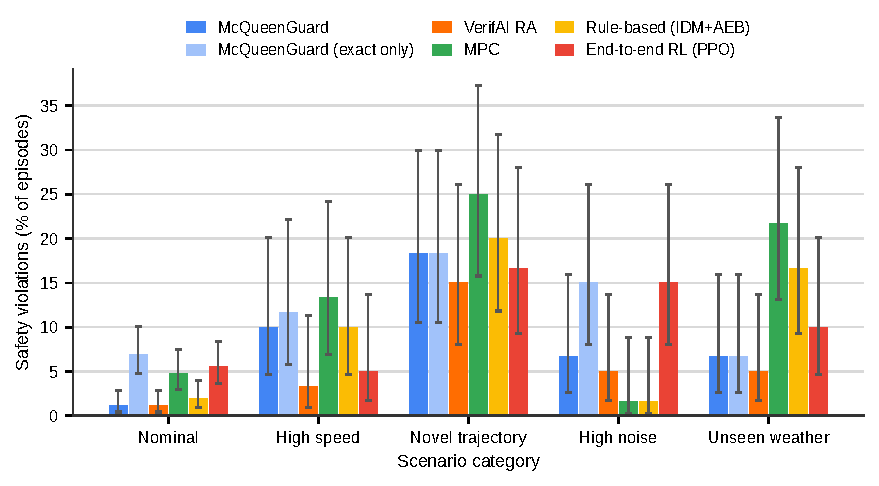
\includegraphics[width=0.92\linewidth]{../figures/fig_c7_safety_by_group.pdf}
\caption{Safety violations (collision or safe-margin violation) per scenario group, with 95\,\% Wilson intervals.}\label{fig:c7a}
\end{figure}
\begin{figure}[h]
\centering
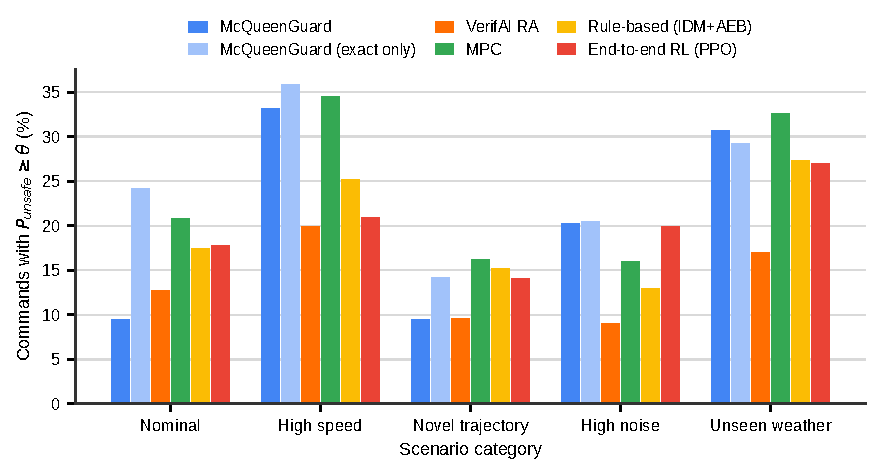
\includegraphics[width=0.92\linewidth]{../figures/fig_c7_risk.pdf}
\caption{Share of audited control commands whose exactly verified 4-s unsafe probability is at least $\theta=0.05$.}\label{fig:c7b}
\end{figure}
\begin{figure}[h]
\centering
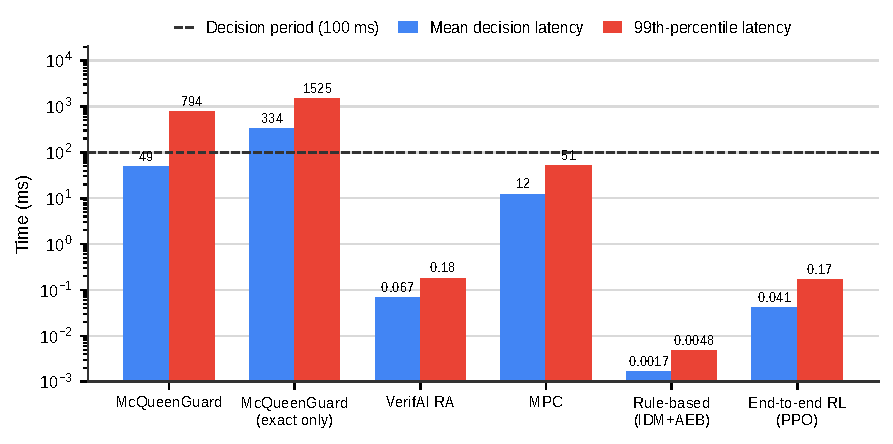
\includegraphics[width=0.92\linewidth]{../figures/fig_c7_latency.pdf}
\caption{Decision latency per method (log scale). McQueenGuard's values include the decisions that fall back to PRISM; a learned
decision alone takes <<us(LB['learned_path']['mean_us'])>> on average (Table~\ref{tab:lat}).}\label{fig:c7c}
\end{figure}

\textbf{Findings.}
<<C7_FINDINGS>>

%-----------------------------------------------------------------------------------------------------
\clearpage
\section*{6.10 \quad Ablation Study and Large-Scale Preservation Analysis}
\addcontentsline{toc}{section}{6.10 Ablation study and large-scale preservation analysis}
\textbf{Ablation.} Table~\ref{tab:abl} and Figure~\ref{fig:abl} report the complete framework, seven reduced variants and an idealised reference
on the same <<N_EP>> scenario instances. Each reduced variant removes one component (the variant ``learned verifier only, $-$ Simplex shield''
removes the admission mechanism, the exact fallback and the shield).

\begin{table}[h]
\centering\small
\caption{Ablation study (<<N_EP>> paired episodes per variant). $p$: exact McNemar test of the safety-violation rate against the complete
framework (all $p<0.05$ remain below 0.05 after Holm correction for the eight comparisons). Decision modes: share of decisions taken by the learned verifier / by exact verification / by the conservative fallback control.}\label{tab:abl}
\begin{adjustbox}{max width=\linewidth}
\begin{tabular}{lccccccccccc}
\toprule
 & Collision & \multicolumn{4}{c}{Safety violation (\%)} & Deadlock & Travel-time & Verified risk & Decision modes & Latency & Deadline \\
\cmidrule(lr){3-6}
Variant & (\%) & all & $p$ & ID & OOD & (\%) & ratio & $\ge\theta$ (\%) & (\%) & mean (ms) & misses (\%) \\
\midrule
<<"\n".join(t_abl)>>
\bottomrule
\end{tabular}
\end{adjustbox}
\par\smallskip\raggedright\footnotesize $^{a}$Non-admitted decisions apply the conservative fallback control (at most reduce speed; emergency
brake if no action is admissible) instead of waiting for PRISM. $^{b}$No margin, no familiarity check, no exact fallback; the Simplex shield is
active. $^{c}$No learned verifier. <<IDEAL_FOOT>>
\end{table}

\begin{figure}[h]
\centering
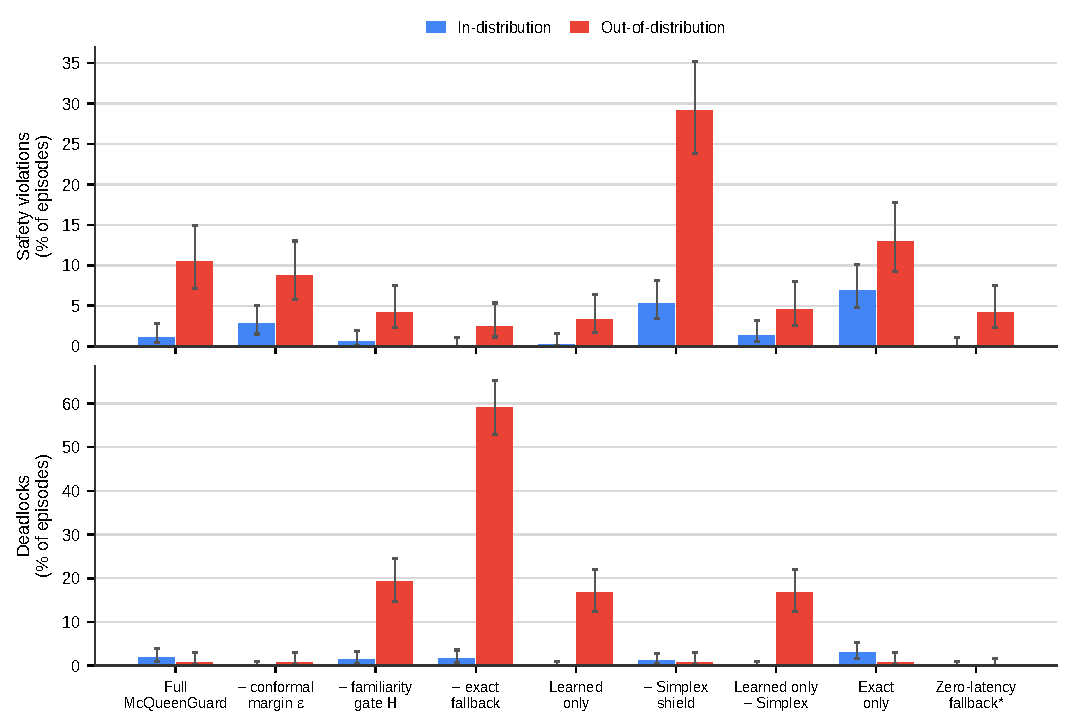
\includegraphics[width=\linewidth]{../figures/fig_r2_ablation.pdf}
\caption{Ablation: safety violations and deadlocks in the in-distribution and out-of-distribution categories (95\,\% Wilson intervals).}\label{fig:abl}
\end{figure}

<<ABL_FINDINGS>>

\textbf{Large-scale preservation analysis.} Table~2 illustrates decision preservation with twelve cases. To provide evidence at scale, every
third decision of the complete framework in all <<N_EP>> episodes was additionally verified exactly for all five actions, outside the timed
decision path (<<f"{n_dec_total:,}">> decisions: <<f"{POL['ID']['full']['n']:,}">> in-distribution and <<f"{POL['OOD']['full']['n']:,}">> out of
distribution). On this decision stream we evaluate four admission policies (Table~\ref{tab:pol}, Figure~\ref{fig:pres}a): no admission rule, the
conformal margin only, the familiarity check only, and both, as in McQueenGuard. A \emph{false admission} is a decision in which a learned result
is admitted although the exact unsafe probability of the admitted action is at least $\theta$; Corollary~1 bounds its probability by $\alpha=5\,\%$.
The counterfactual policies are evaluated on the states visited by the complete framework.

\begin{table}[h]
\centering\small
\caption{Admission policies on <<f"{n_dec_total:,}">> exactly verified decisions. Admitted: share of decisions admitted to the learned verifier;
false admissions in \% of all decisions and of admitted decisions; agreement: admitted learned action equals the exact action.}\label{tab:pol}
\begin{adjustbox}{max width=\linewidth}
\begin{tabular}{lcccccccc}
\toprule
 & \multicolumn{4}{c}{In-distribution} & \multicolumn{4}{c}{Out-of-distribution} \\
\cmidrule(lr){2-5}\cmidrule(lr){6-9}
 & Admitted & \multicolumn{2}{c}{False admissions} & Agreement & Admitted & \multicolumn{2}{c}{False admissions} & Agreement \\
Admission policy & (\%) & (\% dec.) & (\% adm.) & (\%) & (\%) & (\% dec.) & (\% adm.) & (\%) \\
\midrule
<<"\n".join(t_pol)>>
\bottomrule
\end{tabular}
\end{adjustbox}
\end{table}

\begin{table}[h]
\centering\small
\caption{Decision preservation (Theorem~1) on the <<f"{R2['admitted_total']:,}">> admitted decisions. $\varepsilon_U=<<f"{R2['eps_u']:.3f}">>$ is the
split-conformal bound on $\max_a|U(a)-\hat U(a)|$ ($\alpha=0.05$) and $m(x)=\mathcal{T}(k)-2\varepsilon_U$. Regret: mean exact utility loss of
the disagreeing decisions.}\label{tab:th1}
\begin{adjustbox}{max width=\linewidth}
\begin{tabular}{lcccc}
\toprule
Group of admitted decisions & Decisions & Agreement (\%) & Regret & Unsafe admitted actions \\
\midrule
<<TH_ROWS>>
\bottomrule
\end{tabular}
\end{adjustbox}
\end{table}

\begin{figure}[h]
\centering
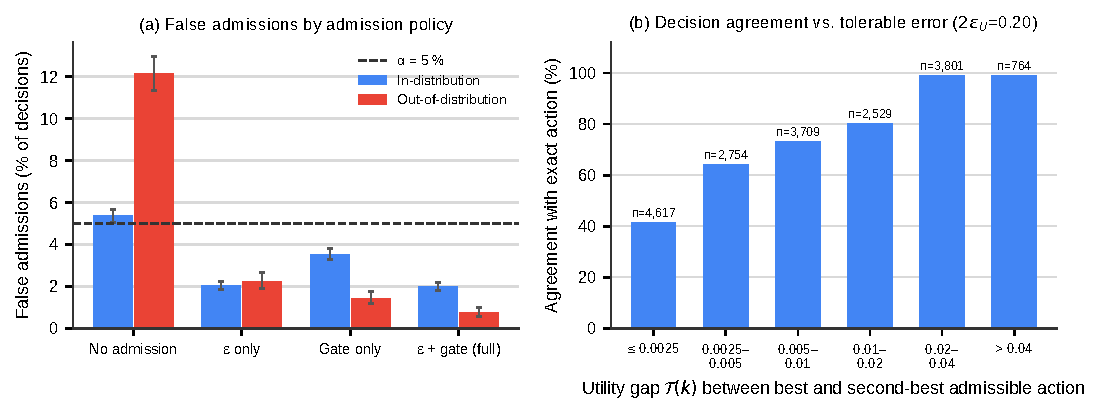
\includegraphics[width=\linewidth]{../figures/fig_r2_preservation.pdf}
\caption{(a) False admissions per decision for four admission policies (95\,\% Wilson intervals). (b) Agreement between the admitted learned
action and the exact action as a function of the utility gap $\mathcal{T}(k)$ (admitted decisions with the same learned and exact admissible set);
the calibrated condition of Theorem~1 requires $\mathcal{T}(k)>2\varepsilon_U$.}\label{fig:pres}
\end{figure}

<<PRES_FINDINGS>>

%-----------------------------------------------------------------------------------------------------
\clearpage
\section*{6.11 \quad Reliability of the Error Bound under Out-of-Distribution Conditions and Latency Breakdown}
\addcontentsline{toc}{section}{6.11 Out-of-distribution reliability and latency breakdown}
\textbf{Error-bound reliability.} Table~\ref{tab:ood} and Figure~\ref{fig:ood} report, for each scenario category, the coverage of the calibrated
margin, the false-admission rate and the fallback rate on the exactly verified decisions of the complete framework, together with the
closed-loop safety outcomes. Coverage is reported for all decisions, for the \emph{risk-relevant} decisions (at least one candidate action with
exact unsafe probability $\ge 10^{-3}$) and for the admitted decisions. The sensor-noise shift study of Section~6.12 complements this analysis
with a gradual shift of the noise distribution.

\begin{table}[h]
\centering\small
\caption{Error-bound coverage, admission and safety outcomes per scenario category (complete framework). The four categories below the line are
out of distribution. False admissions in \% of decisions; ``w/o $\mathcal{H}$'': counterfactual without the familiarity check.}\label{tab:ood}
\begin{adjustbox}{max width=\linewidth}
\begin{tabular}{lcccccccccc}
\toprule
 & Labelled & Familiar & Fallback & \multicolumn{3}{c}{Coverage of $\varepsilon$ (\%)} & \multicolumn{2}{c}{False admissions (\%)} & \multicolumn{2}{c}{Episodes (\%)} \\
\cmidrule(lr){5-7}\cmidrule(lr){8-9}\cmidrule(lr){10-11}
Category & decisions & (\%) & all / risk-rel. & all & risk-relevant & admitted & McQueenGuard & w/o $\mathcal{H}$ & collision & safety viol. \\
\midrule
<<t_cat>>
\bottomrule
\end{tabular}
\end{adjustbox}
\end{table}

\begin{figure}[h]
\centering
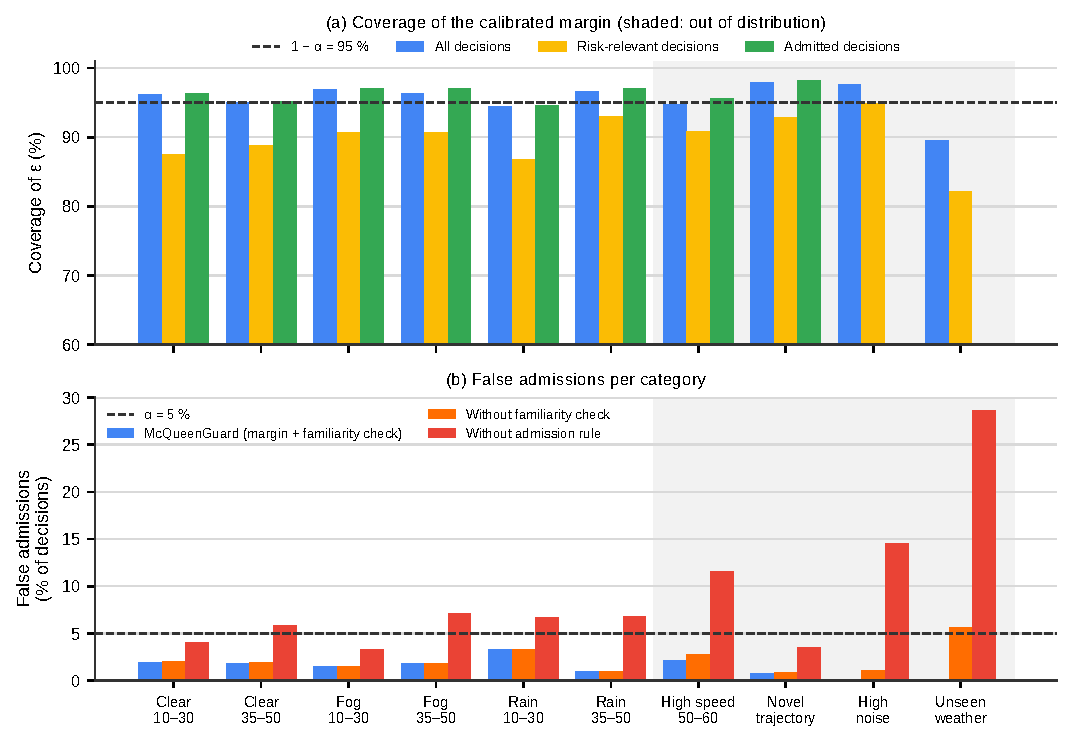
\includegraphics[width=\linewidth]{../figures/fig_r2_ood.pdf}
\caption{(a) Coverage of the calibrated margin per category. (b) False admissions per category for McQueenGuard and for two counterfactual
admission rules evaluated on the same decisions. Shaded: out-of-distribution categories.}\label{fig:ood}
\end{figure}

<<OOD_FINDINGS>>

\textbf{Relation to Table~3.} The fallback rates of Table~\ref{tab:ood} are not directly comparable with those of Table~3. Table~3 counts the
verification mode at the critical decision point of each CARLA scenario run, whereas Table~\ref{tab:ood} counts every decision of an episode,
most of which are routine decisions far from the pedestrian. On risk-relevant decisions, which are closer to the critical decision points, the
testbed fallback rates follow the ordering of Table~3 (clear $<$ fog $<$ rain, higher at higher speed, and 100\,\% under high noise and unseen
weather) at lower absolute values. The exception is the novel-trajectory category (<<f1(FBR['Novel trajectory'])>>\,\% here against 87\,\% in Table~3):
in the testbed, running and occluded pedestrians produce feature values inside the training range, so the familiarity check does not flag them.
This difference indicates that familiarity must be defined on features that capture pedestrian behaviour if novel trajectories are to be routed to
exact verification; as shown above, exact verification would not remove the resulting violations, because they originate in the verification model.

\textbf{Latency breakdown.} Table~\ref{tab:lat} decomposes the decision latency. The runtime rows of Table~4 (2.1\,ms against 148.6\,ms, about
70$\times$) compare the inference time of the learned verifier with the time of one exact verification; they are component times, not the
end-to-end overhead. In the revised Table~4 these rows are labelled ``Learned-verifier inference time'' and ``Exact PRISM verification time per
decision'', and the end-to-end values of Table~\ref{tab:lat} are added.

\begin{table}[h]
\centering\small
\caption{Decomposition of the decision latency (single CPU thread; exact path measured on <<f"{LB['prism']['n']}">> runtime queries with a warm
PRISM server).}\label{tab:lat}
\begin{tabular}{lcc}
\toprule
Component & mean & p99 \\
\midrule
<<t_lat>>
\bottomrule
\end{tabular}
\end{table}

<<LAT_FINDINGS>>

%-----------------------------------------------------------------------------------------------------
\clearpage
\section*{6.12 \quad Embedded Deployment and Sensor-Noise Shift}
\addcontentsline{toc}{section}{6.12 Embedded deployment and sensor-noise shift}
\textbf{Latency, memory and energy of the learned verifier.} The learned verifier was exported to ONNX and measured in four runtimes with one
thread and batch size one (20,000 inferences each; 10,000 for PyTorch); the complete learned decision path was measured on 3,000 recorded runtime observations
from all ten categories (Table~\ref{tab:emb}; the same measurements are decomposed in Table~\ref{tab:lat}). The MLP has <<f"{mod['params']:,}">> parameters and needs <<f"{mod['macs']:,}">> multiply-accumulate operations per
inference.

\begin{table}[h]
\centering\small
\caption{Measured latency of the learned and exact verification paths (single CPU thread). The NumPy, ONNX FP32, learned-path and PRISM rows are the
measurements of Table~\ref{tab:lat}; the PyTorch and INT8 rows come from a separate benchmark run on the same machine.}\label{tab:emb}
\begin{tabular}{lcc}
\toprule
Component & mean & p99 \\
\midrule
<<"\n".join(t_emb)>>
\bottomrule
\end{tabular}
\end{table}

\emph{Memory.} The weights occupy <<f"{mod['fp32_kib']:.1f}">>\,KiB in FP32 (ONNX file <<f"{mod['onnx_fp32_kib']:.1f}">>\,KiB; INT8 file
<<f"{mod['onnx_int8_kib']:.1f}">>\,KiB) and the activations <<mem['mlp_activations_bytes']>>\,bytes. A minimal Python process with ONNX Runtime serving
the INT8 model has a resident set of <<f"{mem['ort_int8_process']:.0f}">>\,MB, of which the inference session accounts for
<<f"{mem['ort_int8_session_increment']:.0f}">>\,MB; the PRISM verification server (Java virtual machine) reaches <<f"{mem['prism_jvm_peak_rss']:.0f}">>\,MB.
Dynamic INT8 quantisation changes the predictions by at most <<f"{E['int8_accuracy']['max_dev_int8_vs_fp32']:.3f}">> (MAE
<<f"{E['int8_accuracy']['mae_fp32']:.4f}">> for FP32 and <<f"{E['int8_accuracy']['mae_int8']:.4f}">> for INT8); after recalibration the INT8 margin is
<<f"{E['int8_accuracy']['eps_int8']:.3f}">> with <<f1(100*E['int8_accuracy']['coverage_int8'])>>\,\% coverage, so the admission mechanism remains valid with a
wider margin. On this x86 CPU the INT8 model is not faster than FP32; its benefit is the smaller model.

\emph{Projection to NVIDIA Jetson AGX Orin.} No Orin board was available. Table~\ref{tab:orin} therefore projects the measured latencies to the Orin
CPU (twelve Arm Cortex-A78AE cores at up to 2.2\,GHz, module power 15--60\,W) with an explicit single-thread slow-down band of 1.5--4$\times$, and
bounds the energy per decision by the module power envelope multiplied by the decision time. This bound is conservative, because the module power
includes idle subsystems.

\begin{table}[h]
\centering\small
\caption{Projected decision latency and energy per decision on Jetson AGX Orin (assumption-based, see text).}\label{tab:orin}
\begin{adjustbox}{max width=\linewidth}
\begin{tabular}{lcccccc}
\toprule
Slow-down & \multicolumn{2}{c}{Learned decision} & \multicolumn{2}{c}{Exact verification} & \multicolumn{2}{c}{Energy per decision, 15\,W / 60\,W (upper bound)} \\
\cmidrule(lr){2-3}\cmidrule(lr){4-5}\cmidrule(lr){6-7}
assumption & mean & p99 & mean & p99 & learned & exact \\
\midrule
<<"\n".join(t_proj)>>
\bottomrule
\end{tabular}
\end{adjustbox}
\end{table}

\textbf{Closed loop under embedded timing.} To test whether the safety results survive slower hardware, <<n_et>> episodes (10 per category, the same
instances as in Section~6.9) were re-run with every measured computation time multiplied by 2.5, the central projection (Table~\ref{tab:et},
Figure~\ref{fig:et}).

\begin{table}[h]
\centering\small
\caption{Testbed timing and embedded timing ($\times$2.5), <<n_et>> paired episodes per method.}\label{tab:et}
\begin{adjustbox}{max width=\linewidth}
\begin{tabular}{lcccccc}
\toprule
 & \multicolumn{3}{c}{Testbed timing} & \multicolumn{3}{c}{Embedded timing ($\times$2.5)} \\
\cmidrule(lr){2-4}\cmidrule(lr){5-7}
Method & latency (ms) & misses (\%) & safety viol. (\%) & latency (ms) & misses (\%) & safety viol. (\%) \\
\midrule
<<"\n".join(t_et)>>
\bottomrule
\end{tabular}
\end{adjustbox}
\end{table}
\begin{figure}[h]
\centering
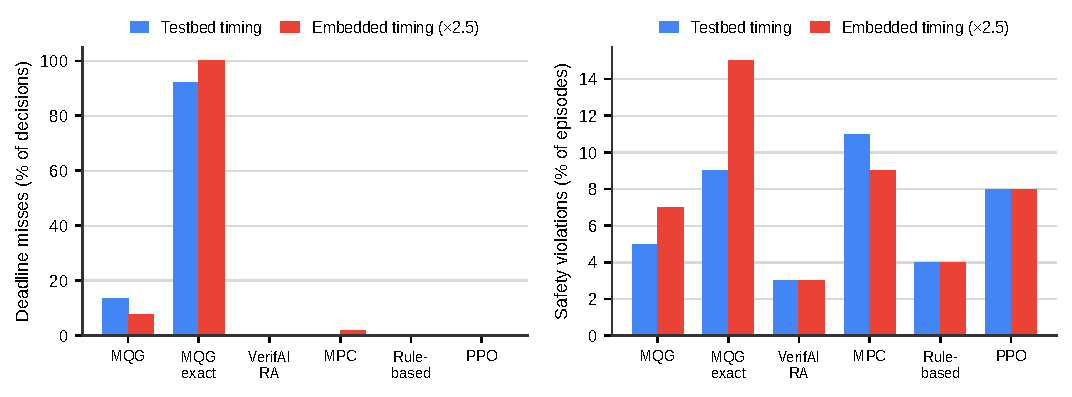
\includegraphics[width=0.95\linewidth]{../figures/fig_c6_embedded_timing.pdf}
\caption{Deadline misses and safety violations with testbed timing and embedded timing (MQG = McQueenGuard).}\label{fig:et}
\end{figure}

<<ET_FINDINGS>>

\textbf{Shift of the sensor-noise distribution (simulation to real).} At test time the perception noise model was replaced by a combined shift of
severity $s\in\{0,0.5,1\}$ that the framework is not told about: Student-$t$ noise with $6-4s$ degrees of freedom and a scale of $1+1.5s$, a
systematic lateral bias of $0.6s$\,m, $25s$\,\% additional drop-outs and $120s$\,ms additional latency. Three mechanisms act under such a shift:
(i) the familiarity check routes unfamiliar feature vectors to exact verification; (ii) the exact results of these fallbacks, together with
shadow audits of 10\,\% of the admitted decisions run outside the critical path, are used to recompute the conformal quantile of Equation~(25)
over a rolling window of the last 200 residuals, without letting $\varepsilon$ fall below its offline value (Algorithm~1, lines~27--28);
(iii) the Simplex shield and the exact fallback remain active regardless of the learned verifier. Table~\ref{tab:ss} and Figure~\ref{fig:ss}
evaluate the admission policies on exactly verified decisions collected under the shift, and Table~\ref{tab:sc} reports the closed-loop outcomes.

\begin{table}[h]
\centering\small
\caption{Decision-stream analysis under the sensor-noise shift. Admission rate / unsafe-admission rate (\% of admitted decisions).}\label{tab:ss}
\begin{adjustbox}{max width=\linewidth}
\begin{tabular}{cccccccc}
\toprule
 & Verified & Coverage of & Familiar & Static margin, & Static margin & + online & $\varepsilon$ after \\
$s$ & decisions & static margin (\%) & (\%) & no check & + check & recalibration & recalibration \\
\midrule
<<"\n".join(t_ss)>>
\bottomrule
\end{tabular}
\end{adjustbox}
\end{table}
\begin{figure}[h]
\centering
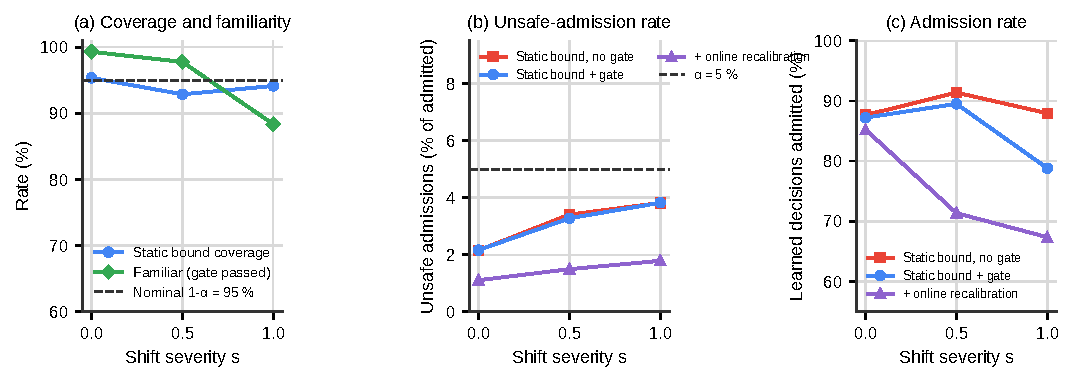
\includegraphics[width=\linewidth]{../figures/fig_c6_shift_stream.pdf}
\caption{Effect of the sensor-noise shift on (a) coverage and familiarity, (b) unsafe-admission rate and (c) admission rate.}\label{fig:ss}
\end{figure}
\begin{table}[h]
\centering\small
\caption{Closed loop under the sensor-noise shift: collision / safety-violation rate (\%), <<n_sc>> episodes per severity and method
(in-distribution categories).}\label{tab:sc}
\begin{tabular}{l<<"c"*len(sevs)>>}
\toprule
Method & <<" & ".join(f"$s={s:.1f}$" for s in sevs)>> \\
\midrule
<<"\n".join(t_sc)>>
\bottomrule
\end{tabular}
\end{table}

<<SHIFT_FINDINGS>>

%-----------------------------------------------------------------------------------------------------
\section*{Revisions of existing text in Sections 5 and 6}
\addcontentsline{toc}{section}{Revisions of existing text in Sections 5 and 6}
<<REVISIONS>>

\section*{6.13 \quad Threats to Validity (additions to the former Section~6.8)}
\addcontentsline{toc}{section}{6.13 Threats to validity (additions)}
<<THREATS>>

\end{document}
